\chapter{Implémentation d'Arcus}

Nous avons choisi de développer le projet Arcus en C++. En effet, le C++ est un langage orienté objet, ce qui correspond à la modélisation objet que nous avons réalisé pour notre application, et multi-plateformes, ce qui nous permettra de porter l'application sur plusieurs systèmes relativement facilement.

Par ailleurs, le C++ est l'un des principaux langages enseignés dans notre formation. Nous possédons donc des acquis avec ce langage, et ce projet nous permet d'en améliorer notre connaissances. Enfin, ce langage jouit d'une communauté importante, de nombreuses bibliothèques ainsi que d'une documentation très complète.

Nous avons choisi d'utiliser C++11, la version de C++ spécifiée par le standard publié en 2012~\parencite{cpp11}. Celle-ci ajoute de nombreuses fonctionnalités au langage et à la bibliothèque standard, entre autres le multi-tâches, les lambdas, les tables de hachage et les expressions régulières.

Nous compilons notre code avec le compilateur Clang, et, pour automatiser la compilation, nous avons utilisé CMake. CMake dispose d'un méta-langage qui permet de produire à la fois des fichiers pour Make, XCode, Visual Studio et d'autres environnements. Il facilite donc le portage.

Ces choix sont résumés dans la table~\ref{table:implementation-tools}.

\section{Mise en place de la communication avec les serveurs}

Pour réaliser le module de communication, nous avons décidé d'utiliser la bibliothèque cURL.\footnote{cURL : \url{https://curl.haxx.se/}} L'utilisation de cette bibliothèque nous permet de bénéficier de sa robustesse, sa simplicité et sa fiabilité. Il s'agit par ailleurs d'une des bibliothèques les plus utilisées pour la communication sur HTTP, notamment utilisée par Adobe, Apple, Microsoft, Mozilla et Spotify~\parencite{curl-companies}. La plupart des problèmes que nous pouvons rencontrer avec cette bibliothèque sont donc déjà documentés.

Nous avons opté pour une implémentation permettant de traiter les requêtes en provenance du module Services de manière asynchrone. Le but est que, pendant l'envoi d'une requête et l'attente de sa réponse, le module puisse continuer d'accepter d'autres requêtes de la part de l'application. Ainsi l'application peut continuer à s'exécuter en attendant le téléversement ou le téléchargement de données vers ou depuis un serveur.

Pour ce faire, nous avons réalisé une implémentation multi-tâches avec deux tâches parallèles : une tâche principale qui reçoit les requêtes et une tâche qui s'occupe de les envoyer et de réceptionner les réponses. Cette implémentation exploite les fonctionnalités de multi-tâches introduites en C++11, en complément de la bibliothèque Boost Thread.~\footnote{Boost Thread : \url{http://www.boost.org/doc/libs/1_64_0/doc/html/thread.html}}

Lorsque la tâche principale reçoit une requête en provenance du module Service, elle l'ajoute dans une file d'attente des requêtes à envoyer et continue son exécution. En parallèle, la tâche d'envoi et de réception boucle en permanence en attendant que des requêtes arrivent dans la file d'attente. Elle les envoie alors une par une aux serveurs distants et réceptionne les réponses. Lorsqu'une réponse est reçue par la tâche d'envoi et de réception, celle-ci est transmise à la tâche principale via une promesse. La figure~\ref{fig:implementation-http-thread}, donne un exemple de comportement de ces deux tâches.

\begin{figure}[h]
    \centering
    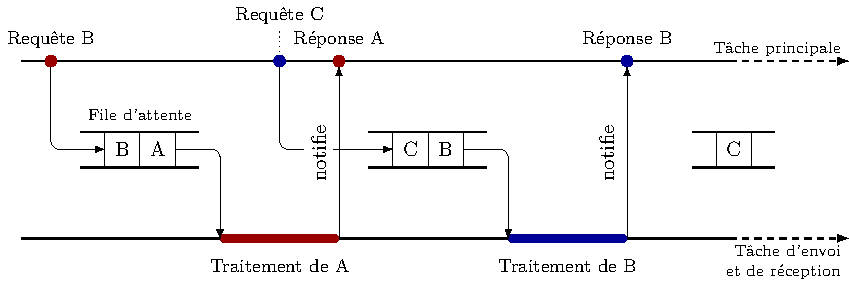
\includegraphics{figures/implementation-thread}
    \caption{\textbf{Exemple de comportement des deux tâches lors d'envois de requêtes.} La tâche principale reçoit une requête supplémentaire C pendant que la tâche d'envoi et de réception est en train de traiter la requête A.}
    \label{fig:implementation-http-thread}
\end{figure}

À chaque envoi de requête, la bibliothèque cURL ouvre une nouvelle connexion au serveur demandé. Ce comportement peut se révéler inefficace notamment si plusieurs requêtes vers le même serveur sont envoyées à la suite. Pour limiter ce problème, nous avons créé une classe de piscine~\emph{(pool)} permettant de mutualiser les ressources et notamment de garder la même connexion ouverte pour plusieurs requêtes vers le même serveur dans un intervalle de temps court.

L'annexe~\ref{appendix:code-sender} présente les principaux extraits du code gérant la synchronisation entre les deux tâches et l'utilisation de la bibliothèque cURL. La figure~\ref{fig:implementation-http-exemple} montre un exemple d'utilisation du module comme il pourrait l'être dans le module Services.

\begin{figure}[h!]
    \begin{lstlisting}[language=C++]
HTTP::Request req = HTTP::Request()
    .setUrl("https://fr.wikipedia.org/wiki/Wikip%C3%A9dia:Accueil_principal")
    .setVerb(HTTP::Verb::GET);

HTTP::Sender sender;
sender.send(req, &std::cout).get();
    \end{lstlisting}
    \caption{\textbf{Exemple d'utilisation du module HTTP pour envoyer une requête.} Dans cet exemple, le contenu de la page d'accueil de Wikipédia est téléchargé et affiché la sortie standard. Grâce au travail réalisé dans ce module, nous sommes en mesure d'écrire un code concis de haut niveau pour envoyer des requêtes HTTP et récupérer leur réponse.}
    \label{fig:implementation-http-exemple}
\end{figure}

\section{Création de l'interface commune aux services}

L'objectif du module Services est de fournir une abstraction de la communication avec les interfaces des services de stockage. Pour fournir cette abstraction, nous avons implémenté une classe pour chaque service de stockage. Chacune de ces classes réalise l'interface présentée dans la partie conception.

Dans ces classes, chaque action abstraite requise par l'interface, comme l'ajout d'un fichier ou la récupération du quota, est «~traduite~» en une requête ou série de requêtes permettant de réaliser cette action sur le service. Une fois la réponse du serveur du service reçue, celle-ci est transformée dans les structures de données utilisées par notre application.

L'implémentation de ce module ne présente pas de complexité technique particulière, si ce n'est celle de manier correctement le concept de promesses. Cette simplicité est due au fait que les détails d'implémentation de la communication sont cachés dans le module HTTP. L'annexe~\ref{appendix:code-service} montre quelques exemples de traduction des actions pour l'A.P.I. de Dropbox.

Vu de l'extérieur de ce module, la communication avec l'un ou l'autre des services supportés est totalement transparente. Cela nous permet, dans les autres modules, de manipuler un service de façon abstraite sans craindre de devoir modifier le code en cas d'ajout d'un nouveau service.

\section{Formats de stockage des configurations}

Nous avons choisi, pour stocker la configuration synchronisée, une base de données SQLite~3.\footnote{SQLite~3 : \url{https://www.sqlite.org/}} Nous avons donc converti notre modèle entité-association, présenté dans la partie conception, en modèle relationnel, décrit dans la figure~\ref{fig:implementation-config-bd}. Nous avons choisi la bibliothèque SQLite~3 car elle dispose d'une A.P.I. simple d'utilisation, et que les bases de données produites sont contenues dans un unique fichier, ce qui simplifie grandement leur synchronisation avec les différents services.

\begin{figure}[h]
    \begin{lstlisting}[escapeinside={(*}{*)}]
Entry((*\uline{id}*), name, type, (*\dashuline{parent}*))
Chunk((*\uline{id}*), hash, order, (*\dashuline{File.id}*))
ChunkService((*\dashuline{Chunk.id}*), (*\dashuline{Service.id}*))
Service((*\uline{id}*), provider, auth)
    \end{lstlisting}
    \caption{\textbf{Modèle relationnel de la base de données.}}
    \label{fig:implementation-config-bd}
\end{figure}

En raison de la simplicité de la structure de la configuration locale de notre application, nous avons choisi un format plus léger qu'une base de données : le \emph{JavaScript Object Notation} (JSON, \cite{ecma404}). Ce format a l'avantage d'être simple et compréhensible par un humain. Pour lire et écrire les fichiers JSON, nous utilisons la bibliothèque \texttt{nlohmann::json}\footnote{\texttt{nlohmann::json} : \url{https://github.com/nlohmann/json}}. La figure~\ref{fig:conception-local} présente le format de ce fichier.

\begin{figure}[h]
    \begin{verbatim}{
    "monitored_directories": {
        "ID-ZONE-1": "/chemin/zone-1/",
        "ID-ZONE-2": "/chemin/zone-2/",
        "ID-ZONE-3": "/chemin/zone-3/"
    }
}\end{verbatim}
    \caption{\textbf{Format du fichier de configuration local.} Sous la clef \texttt{monitored\_directories} se trouve un dictionnaire associant les identifiants des zones de synchronisation aux chemins des répertoires sur lesquels elles sont attachées.}
    \label{fig:conception-local}
\end{figure}

Pour les identifiants dans les fichiers de configuration, nous utilisons des \emph{Universally Unique IDentifier} (UUID). Pour les générer, nous utilisons la bibliothèque Boost UUID~\footnote{Boost UUID : \url{http://www.boost.org/doc/libs/1_64_0/libs/uuid/uuid.html}} qui est compatible avec la majorité des systèmes d'exploitation.

\section{Détection des changements dans le système de fichiers}

Afin de détecter l'ajout, la suppression ou la mise à jour des fichiers locaux, nous utilisons fswatch\footnote{\texttt{fswatch} : \url{http://emcrisostomo.github.io/fswatch/}}. Cette bibliothèque a le grand avantage d'abstraire derrière une A.P.I. C++ de haut niveau les mécanismes très divers des différents systèmes d'exploitation permettant l'observation des changements effectués dans le système de fichiers. Son utilisation permettra d'adapter Arcus sur plusieurs systèmes plus facilement.

\begin{table}[h]
    \centering
    \begin{tabular}{lll}
        & \textbf{Fonction} & \textbf{Outil}\\
        \toprule
        \textbf{Code} & Langage & C++11\\
        \cmidrule{2-3}
        & Compilateur & Clang\\
        \cmidrule{2-3}
        & Construction automatisée & CMake\\
        \midrule
        \textbf{Bibliothèques} & Requêtes HTTP & cURL\\
        \cmidrule{2-3}
        & Base de données & SQLite~3\\
        \cmidrule{2-3}
        & Interprétation JSON & \texttt{nlohmann::json}\\
        \cmidrule{2-3}
        & Observation arborescence & fswatch\\
        \cmidrule{2-3}
        & Chemins et système de fichiers & Boost Filesystem\\
        \cmidrule{2-3}
        & Identifiants uniques & Boost UUID\\
        \cmidrule{2-3}
        & Threads & Bibliothèque standard et Boost Thread\\
        \bottomrule
    \end{tabular}

    \caption{\textbf{Résumé des technologies choisies pour l'implémentation.}}
    \label{table:implementation-tools}
\end{table}
